\documentclass{cours}
\usepackage{pgfplots}
\usepackage{multicol}
\usepackage{calc}
\usepackage{esvect}
\usepackage{tikz-3dplot} 
\usetikzlibrary{patterns}
\begin{document}
\setcounter{chapter}{9}
\chapter{Cinématique}
\section{Description du mouvement d'un point}%
\label{sec:description_du_mouvement_d_un_point}

\subsection{Référentiel d'observation}%
\label{sub:referentiel_d_observation}

Le mouvement d'un point matériel dépend de celui de l'observateur. Donc avant de décrire le mouvement d'un point, il faut définir le \emph{référentiel d'observation}.

\begin{definition}
Un \textbf{référentiel} $\mathcal{R}$ est défini par une origine $O$ à laquelle on attache trois axes $Ox$, $Oy$, $Oz$ non coplanaires fixes. On lui associe une horloge qui permet de repérer les événements dans le temps. 
\end{definition}

En mécanique classique, on fait les hypothèses suivantes :
\begin{itemize}
  \item L'espace possède 3 dimensions et est considéré comme euclidien. 
  \item Le temps est considéré comme absolu et ne dépend pas du référentiel choisi. Toutes les horloges vont à la même vitesse et un intervalle de temps entre deux événements sera le même quels que soient les référentiels d'observation de ces événements.
  \item La distance entre deux points de l'espace est absolue et ne dépend pas du référentiel dans lequel on la mesure. 
\end{itemize}

Ces trois hypothèses ne sont plus valables dans les théories relativistes de la mécanique (relativité restreinte et générale).

Dans le référentiel $\mathcal{R}$, la position d'un point $M$ est repérée par son \textbf{vecteur position} $\vv{OM}$. 
\begin{itemize}
  \item Le \textbf{vecteur vitesse} du point $M$ est défini comme $\vv*{v}{M} = \dt{\vv{OM}}$  
  \item Le \textbf{vecteur accélération} du point $M$ est défini comme $\vv*{a}{M} = \ddt{\vv{OM}}$  
\end{itemize}

Exemples de référentiels :
\begin{itemize}
  \item \textbf{Référentiel du laboratoire : }$O$ est dans un coin de la pièce et $x$, $y$ $z$ sont suivant trois arêtes perpendiculaires de la pièce.
  \item \textbf{Référentiel terrestre : } $O$ est au centre de la Terre et $x$, $y$, $z$ dirigés vers des points fixes à la surface de la Terre.
  \item \textbf{Référentiel géocentrique : } $O$ est au centre de la Terre et $x$, $y$, $z$ dirigés vers des étoiles lointaines fixes.
  \item \textbf{Référentiel héliocentrique : } $O$ est au centre du Soleil et $x$, $y$, $z$ dirigés vers des étoiles lointaines fixes.
\end{itemize}

\subsection{Systèmes de coordonnées}%
\label{sub:systemes_de_coordonnees}
Pour décrire quantitativement le mouvement d'un point $M$ dans le référentiel choisi, il faut utiliser un \textbf{système de coordonnées} qui permet d'exprimer la position de $M$ par des nombres. 

\subsubsection{Système de coordonnées cartésiennes}%
\label{ssub:systeme_de_coordonnees_cartesiennes}

On donne trois vecteurs $\vex, \vey, \vez$ unitaires orthogonaux, fixes dans le référentiel d'études. La position d'un point $M$ est repérée par les trois coordonnées $x$, $y$, et $z$ du vecteur $\vv{OM} = x \vex + y \vey  + z \vez$.   

\noindent\begin{minipage}{\linewidth}
\noindent\begin{minipage}{0.5\linewidth}
%Coordonnées cartésiennes
\begin{center}
\tdplotsetmaincoords{60}{110}
\begin{tikzpicture}[scale=4,tdplot_main_coords]
  %tikz meca
\pgfmathsetmacro{\xvec}{.6}
\pgfmathsetmacro{\yvec}{.6}
\pgfmathsetmacro{\zvec}{.8}


\coordinate (O) at (0,0,0);


\foreach \x in {0.1, 0.2, ..., 1}{
  \draw[thin, gray!50] (\x,0,0) -- (\x,1,0);
  \draw[thin, gray!50] (\x,0,0) -- (\x,0,1);
  \draw[thin, gray!50] (0,\x,0) -- (1,\x,0);
  \draw[thin, gray!50] (0,\x,0) -- (0,\x,1);
  \draw[thin, gray!50] (0,0,\x) -- (1,0,\x);
  \draw[thin, gray!50] (0,0,\x) -- (0,1,\x);
}
%Axes
\draw[thick,-Stealth] (0,0,0) -- (1,0,0) node[anchor=north east]{$x$};
\draw[thick,-Stealth] (0,0,0) -- (0,1,0) node[anchor=north west]{$y$};
\draw[thick,-Stealth] (0,0,0) -- (0,0,1) node[anchor=south]{$z$};

\draw (O) node[above left]{$O$};
\coordinate(M) at (\xvec,\yvec,\zvec);

\draw[-stealth, thick] (O) -- (M) node[above left]{$M$}; 

\tdplotsetrotatedcoordsorigin{(M)}
%trièdre local
\draw[-latex] (M)
-- ++(.3,0,0) node[anchor=north]{$\vv*{e}{x}$};
\draw[-latex] (M)
-- ++(0,.3,0) node[anchor=west]{$\vv*{e}{y}$};
\draw[-latex] (M)
-- ++(0,0,.3) node[anchor=south]{$\vv*{e}{z}$};


%coordonnées
\draw[dashed] (\xvec, 0,0) -- (\xvec, \yvec, 0) node[midway,circle, fill=white, fill opacity=0.8, text opacity=1]{$y$};
\draw[dashed] (0, \yvec,0) -- (\xvec, \yvec, 0) node[midway,circle, fill=white, fill opacity=0.8, text opacity=1]{$x$};
\draw[dashed] (\xvec, \yvec,0) -- (M) node[midway,circle, fill=white, fill opacity=0.8, text opacity=1]{$z$};


\end{tikzpicture}
\end{center}
\end{minipage}%
\begin{minipage}{0.5\linewidth}
%Coordonnées cartésiennes déplacement élémentaire
\begin{center}
\tdplotsetmaincoords{60}{110}
\begin{tikzpicture}[scale=4,tdplot_main_coords]
  %tikz meca

\pgfmathsetmacro{\xvec}{.6}
\pgfmathsetmacro{\yvec}{.6}
\pgfmathsetmacro{\zvec}{.8}

\coordinate (O) at (0,0,0);


\foreach \x in {0.1, 0.2, ..., 1}{
  \draw[thin, gray!50] (\x,0,0) -- (\x,1,0);
  \draw[thin, gray!50] (\x,0,0) -- (\x,0,1);
  \draw[thin, gray!50] (0,\x,0) -- (1,\x,0);
  \draw[thin, gray!50] (0,\x,0) -- (0,\x,1);
  \draw[thin, gray!50] (0,0,\x) -- (1,0,\x);
  \draw[thin, gray!50] (0,0,\x) -- (0,1,\x);
}
%Axes
\draw[thick,-Stealth] (0,0,0) -- (1,0,0) node[anchor=north east]{$\vex $};
\draw[thick,-Stealth] (0,0,0) -- (0,1,0) node[anchor=north west]{$\vey $};
\draw[thick,-Stealth] (0,0,0) -- (0,0,1) node[anchor=south]{$\vez $};

\draw (O) node[above left]{$O$};
\coordinate(M) at (\xvec,\yvec,\zvec);

\draw[-stealth, thick] (O) -- (M) node[above left]{$M$}; 
\draw[-stealth, thick] (M) -- ++(0.6, 0.4, 0.5) node[above]{\scriptsize$\D \vv{OM}$}; 

\tdplotsetrotatedcoordsorigin{(M)}
%trièdre local


\draw[dashed, gray] (\xvec, 0,0) -- (\xvec, \yvec, 0) node[midway,circle, fill=white, fill opacity=0.8, text opacity=1, inner sep=0]{$y$};
\draw[dashed, gray] (0, \yvec,0) -- (\xvec, \yvec, 0) node[midway,circle, fill=white, fill opacity=0.8, text opacity=1, inner sep=0]{$x$} ;
\draw[dashed, gray] (\xvec, \yvec,0) -- (M) node[pos=0.4,circle, fill=white, fill opacity=0.8, text opacity=1, inner sep=0]{$z$};

\draw[dashed] (M) -- ++(.6,0,0) node[midway,circle, fill=white, fill opacity=0.8, text opacity=1, inner sep=0, sloped]{\scriptsize $\D x$} 
-- ++(0,0.4,0) node[midway,circle, fill=white, fill opacity=0.8, text opacity=1, inner sep=0, sloped]{\scriptsize $\D y$} 
-- ++(0,0,0.5) node[midway,circle, fill=white, fill opacity=0.8, text opacity=1, inner sep=0, sloped]{\scriptsize $\D z$};
%\draw[-latex] (M)
%-- ++(0,.3,0) node[anchor=west]{$\vv*{e}{y}$};
%\draw[-latex] (M)
%-- ++(0,0,.3) node[anchor=south]{$\vv*{e}{z}$};




\end{tikzpicture}
\end{center}
\end{minipage}
\captionof{figure}{Système de coordonnées cartésiennes.}
\end{minipage}

Comme les vecteurs de base sont fixes, les vecteurs vitesse et accélération sont : 
\begin{equation}
\vv{v} = \dt{\vv{OM}} = \dot{x}\vex +\dot{y}\vey +\dot{z}\vez \quad \text{et}\quad \vv{a} = \ddt{OM} = \ddot{x}\vex  + \ddot{y}\vey +\ddot{z}\vez
\end{equation}


Si on augmente les coordonnées $x$, $y$, $z$ de respectivement $\D x$, $\D y$ et $\D z$ alors le point $M$ se déplace de 
\begin{equation}
\D \vv{OM} = \D x \vex +\D y \vey + \D z \vez , 
\end{equation}




c'est le vecteur \textbf{déplacement élémentaire}. Le trièdre $(\vex, \vey, \vez)$ est appelé \textbf{trièdre local} associé au point $M$. On peut retrouver l'expression du vecteur vitesse car $\vv{v} = \dt{\vv{OM}}$. 


\subsubsection{Système de coordonnées cylindriques}%
\label{ssub:systeme_de_coordonnees_cylindriques}
La position du point $M$ est donnée par sa distance $r$ à l'axe $z$, sont altitude $z$ par rapport au plan $(x, y)$ et l'angle orienté $\theta$ entre la direction $(Ox)$ et la direction $\vv{OM'}$ où $M'$ est le projeté orthogonal de $M$ sur le plan $(x, y)$.

On construit le \textbf{trièdre local} $(\ver, \vet, \vez)$ de la manière suivante :
\begin{itemize}
  \item Lorsque $r$ augmente de $\D r$ (infiniment petit), le point $M$ se déplace  de $\D r$ suivant $\ver$.   
  \item Lorsque $\theta$ augmente de $\D \theta$ (infiniment petit), le point $M$ se déplace de $r\D \theta$ suivant $\vet$.   
  \item Lorsque $z$ augmente de $\D z$ (infiniment petit), le point $M$ se déplace de $\D z$ suivant $\vez$.   
\end{itemize}

On a alors le déplacement élémentaire :
\begin{equation}
d \vv{OM} = \D r  \ver + r\D \theta \vet + \D z \vez \end{equation}
 
\noindent\begin{minipage}{\linewidth}
\noindent\begin{minipage}{0.5\linewidth}
\begin{center}
%Coordonnées cylindriques
\tdplotsetmaincoords{60}{110}
\begin{tikzpicture}[scale=5,tdplot_main_coords]
  %tikz meca

%
\pgfmathsetmacro{\rvec}{.8}
\pgfmathsetmacro{\thetavec}{60}
\pgfmathsetmacro{\zvec}{0.8}
%
\coordinate (O) at (0,0,0);


\foreach \vtheta in {0, 10, ..., 90}{
  \draw[thin, gray!50,] ({\rvec*cos(\vtheta)},{\rvec*sin(\vtheta)},0) -- ++(0,0,1);
}
\foreach \vz in {0, 0.1, ...,1.01}{
  \tdplotsetrotatedcoords{0}{0}{0}
  %\tdplotsetrotatedcoordsorigin{(0,0,{\rvec*(1-cos(\vtheta))}}
  \draw[thin, gray!50] (\rvec,0,\vz) arc (0:90:\rvec);
}
  \draw[thin, gray!50] (\rvec,0,1) -- (0,0,1);
  \draw[thin, gray!50] (0, \rvec,1) -- (0,0,1);
%Axes
\draw[thick,-Stealth] (0,0,0) -- (1,0,0) node[anchor=north east]{$x$};
\draw[thick,-Stealth] (0,0,0) -- (0,1,0) node[anchor=north west]{$y$};
\draw[thick,-Stealth] (0,0,0) -- (0,0,1) node[anchor=south]{$z$};


\draw (O) node[above left]{$O$};

% Point M
\coordinate (M) at ({\rvec*cos(\thetavec)},{\rvec*sin(\thetavec)},\zvec);
\coordinate (Mxy) at ({\rvec*cos(\thetavec)},{\rvec*sin(\thetavec)},0);
\draw[-stealth, thick] (O) -- (M) node[above left]{$M$};
\draw[dashed] (M) -- (Mxy)node[midway, fill=white, fill opacity=0.8, text opacity=1, circle] {$z$};
\draw[dashed] (Mxy) node[right] {M'}-- (O) node[midway, fill=white, fill opacity=0.8, text opacity=1, circle] {$r$} ;
\draw[-latex] (0.5, 0, 0) arc (0:60:0.5) node[midway, below, fill=white, fill opacity=0.8, text opacity=1, circle] {$\theta$};

%trièdre local
\pgfmathsetmacro{\rvec}{.8}
\pgfmathsetmacro{\thetavec}{60}
\pgfmathsetmacro{\zvec}{0.8}

\draw[-latex] (M) -- ++ ({0.3*cos(\thetavec)},{0.3*sin(\thetavec)},0) node[anchor=north west]{$\vv*{e}{r}$};
\draw[-latex] (M) -- ++ ({-0.3*sin(\thetavec)},{0.3*cos(\thetavec)},0) node[anchor=west]{$\vv*{e}{\theta}$};
\draw[-latex] (M) -- ++ (0,0,0.3) node[anchor=north west]{$\vv*{e}{z}$};

\end{tikzpicture}
\end{center}
\end{minipage}%
\begin{minipage}{0.5\linewidth}
\begin{center}
%Coordonnées cylindriques déplacement élémentaire
\tdplotsetmaincoords{60}{110}
\begin{tikzpicture}[scale=5,tdplot_main_coords]

%
\pgfmathsetmacro{\rvec}{.8}
\pgfmathsetmacro{\thetavec}{40}
\pgfmathsetmacro{\zvec}{0.8}
%
\coordinate (O) at (0,0,0);


\foreach \vtheta in {0, 10, ..., 90}{
  \draw[thin, gray!50,] ({\rvec*cos(\vtheta)},{\rvec*sin(\vtheta)},0) -- ++(0,0,1);
}
\foreach \vz in {0, 0.1, ...,1.01}{
  \tdplotsetrotatedcoords{0}{0}{0}
  %\tdplotsetrotatedcoordsorigin{(0,0,{\rvec*(1-cos(\vtheta))}}
  \draw[thin, gray!50] (\rvec,0,\vz) arc (0:90:\rvec);
}
  \draw[thin, gray!50] (\rvec,0,1) -- (0,0,1);
  \draw[thin, gray!50] (0, \rvec,1) -- (0,0,1);
%Axes
\draw[thick,-Stealth] (0,0,0) -- (1,0,0) node[anchor=north east]{$x$};
\draw[thick,-Stealth] (0,0,0) -- (0,1,0) node[anchor=north west]{$y$};
\draw[thick,-Stealth] (0,0,0) -- (0,0,1) node[anchor=south]{$z$};


\draw (O) node[above left]{$O$};

% Point M
\coordinate (M) at ({\rvec*cos(\thetavec)},{\rvec*sin(\thetavec)},\zvec);
\coordinate (M2) at ({(\rvec+0.2)*cos(50)},{(\rvec+0.2)*sin(50)},{\zvec+0.2});
\coordinate (Mxy) at ({\rvec*cos(\thetavec)},{\rvec*sin(\thetavec)},0);
\draw[-stealth, thick] (O) -- (M) node[left]{$M$};
\draw[-stealth, thick] (M) -- (M2) node[midway, sloped, above]{\scriptsize $\D \vv{OM}$};
\draw[dashed] (M) -- (Mxy)node[midway, fill=white, fill opacity=0.8, text opacity=1, circle] {$z$};
\draw[dashed] (Mxy) node[below left] {M'}-- (O) node[pos=0.7, fill=white, fill opacity=0.8, text opacity=1, circle] {$r$} ;
\draw[dashed] (O) -- (50:\rvec) ;

\draw[-latex] (\rvec, 0, 0) arc (0:\thetavec:\rvec) node[midway, below, fill=white, fill opacity=0.8, text opacity=1, circle] {$\theta$} ;

\draw[-latex] (\thetavec:\rvec) arc(\thetavec:50:\rvec) node[midway,below,   circle] {\scriptsize $\D \theta$};

\draw[-latex] (M) -- ++ ({0.3*cos(\thetavec)},{0.3*sin(\thetavec)},0) node[anchor=north west]{$\vv*{e}{r}$};
\draw[-latex] (M) -- ++ ({-0.3*sin(\thetavec)},{0.3*cos(\thetavec)},0) node[anchor=west]{$\vv*{e}{\theta}$};
\draw[-latex] (M) -- ++ (0,0,0.3) node[anchor=north west]{$\vv*{e}{z}$};

\draw[-|, dashed] (M) -- ++(0,0,0.2) node[midway, fill=white, inner sep=0]{\scriptsize $\D z$};
\draw[-|, dashed] (M) -- ++ ({0.2*cos(\thetavec)},{0.2*sin(\thetavec)},0) node[midway, fill=white, inner sep=0]{\scriptsize $\D r$};

%trièdre local


\end{tikzpicture}
\end{center}
\end{minipage}
\begin{center}
\captionof{figure}{Système de coordonnées cylindriques.}
\end{center}
\end{minipage}
Le vecteur position est $\vv{OM} = r\ver + z\vez$. On déduit le vecteur vitesse à partir du déplacement élémentaire :
\begin{equation}
v = \dt{\vv{OM}} = \dot{r}\ver + r \dot{\theta}\vet + \dot{z}\vez
\end{equation}


On en déduit l'égalité importante $\dt{\ver} = \dot{\theta}\vet$. On peut aussi montrer que $\dt{\vet} = -\dot{\theta}\ver$. Cela nous permet de calculer l'expression du vecteur accélération :

\begin{equation}
\vv{a} = \ddt{\vv{OM}} = (\ddot{r}-r \dot{\theta}^2)\ver + (2 \dot{r}\dot{\theta} + r \ddot{\theta})\vet + \ddot{z}\vez
\end{equation}

\begin{loi}{À retenir}
  En coordonnées cylindriques, les dérivées temporelles des vecteurs $\ver$ et $\vet$ sont
  \begin{equation}
    \dt{\ver} = \dot{\theta}\vet \quad \text{et} \quad \dt{\vet} = -\dot{\theta}\ver
  \end{equation}
\end{loi}



\subsubsection{Système de coordonnées sphériques}%
\label{ssub:systeme_de_coordonnees_sphériques}

Dans un système de coordonnées sphériques, le point $M$ est repéré par :
\begin{itemize}
  \item Sa distance $r$ à l'origine ;
  \item l'angle orienté $\theta$ (colatitude) entre l'axe $(Oz)$ et le vecteur $\vv{OM}$ ;
  \item l'angle $\varphi$ (longitude) entre l'axe $(Ox)$ et le vecteur $\vv{OM'}$, où $M'$ est le projeté orthogonal de $M$ sur le plan $(x, y)$.  

\end{itemize}

\begin{center}
%Coordonnées sphériques
\tdplotsetmaincoords{60}{110}
\begin{tikzpicture}[scale=5,tdplot_main_coords]

%
\pgfmathsetmacro{\rvec}{.8}
\pgfmathsetmacro{\thetavec}{30}
\pgfmathsetmacro{\phivec}{60}
%
\coordinate (O) at (0,0,0);


\foreach \vphi in {0, 15, ..., 90}{
  \tdplotsetthetaplanecoords{\vphi}
  \draw[thin, gray!50,tdplot_rotated_coords] (\rvec,0,0) arc (0:90:\rvec);
}
\foreach \vtheta in {0, 15, ..., 90}{
  \tdplotsetrotatedcoords{0}{0}{0}
  %\tdplotsetrotatedcoordsorigin{(0,0,{\rvec*(1-cos(\vtheta))}}
  \draw[thin, gray!50] ({\rvec*sin(\vtheta)},0,{\rvec*cos(\vtheta)}) arc (0:90:{\rvec*sin(\vtheta)});
}
%Axes
\draw[thick,-Stealth] (0,0,0) -- (1,0,0) node[anchor=north east]{$x$};
\draw[thick,-Stealth] (0,0,0) -- (0,1,0) node[anchor=north west]{$y$};
\draw[thick,-Stealth] (0,0,0) -- (0,0,1) node[anchor=south]{$z$};


\draw (O) node[above left]{$O$};

% Point M
\tdplotsetcoord{M}{\rvec}{\thetavec}{\phivec}
\draw[-stealth, thick] (O) -- (M) node[above left]{$M$} node[midway, sloped, below]{$r$} ;
\draw[dashed,] (O) -- (Mxy) node[below]{$M'$} ;
\draw[dashed,] (M) -- (Mxy);

% Angle Phi
\tdplotdrawarc[-latex]{(O)}{0.2}{0}{\phivec}{anchor=north}{$\varphi$}
\tdplotsetthetaplanecoords{\phivec}
%Angle Theta
\tdplotdrawarc[tdplot_rotated_coords, -latex]{(0,0,0)}{0.5}{0}%
{\thetavec}{anchor=south west}{$\theta$}


\tdplotsetrotatedcoords{\phivec}{\thetavec}{0}
\tdplotsetrotatedcoordsorigin{(M)}

%trièdre local
\draw[tdplot_rotated_coords,-latex] (0,0,0)
-- (.3,0,0) node[anchor=north west]{$\vv*{e}{\theta}$};
\draw[tdplot_rotated_coords,-latex] (0,0,0)
-- (0,.3,0) node[anchor=west]{$\vv*{e}{\varphi}$};
\draw[tdplot_rotated_coords,-latex] (0,0,0)
-- (0,0,.3) node[anchor=south]{$\vv*{e}{r}$};

\end{tikzpicture}
\captionof{figure}{Système de coordonnées sphériques.}
\end{center}

Dans ce cas, le vecteur position est $\vv{OM} = r\ver$, et le vecteur déplacement élémentaire est 
\begin{equation}
\D \vv{OM} = \D r\ver + r\D \theta \vet + r\sin(\theta)\D \varphi\vep
\end{equation}

Dont on peut déduire l'expression du vecteur vitesse  
\begin{equation}
  \vv{v} = \dt{OM} = \dt{r}\ver + r\dt{\theta} \vet + r\sin(\theta)\dt{\varphi}\vep
\end{equation}

\subsubsection{Système de coordonnées adapté}%
\label{ssub:systeme_de_coordonnees_adapte}
Pour traiter un problème de mécanique, il faudra essayer de choisir le système de coordonnées le plus adapté. Pour celà on peut regarder les \textbf{degrés de liberté} du système. Par exemple :

\begin{itemize}
  \item Lorsque la distance d'un point à un axe est fixe, on utilisera le système de coordonnées cylindriques ;
  \item lorsqu'un point est astreint à se déplacer suivant un axe, on utilisera le système de coordonnées cartésiennes ;
  \item Lorsque le distance du point étudié à un point particulier de l'espace est constante, on utilisera les coordonnées sphériques.
\end{itemize}


\section{Exemples de mouvements ponctuels}%
\label{sub:exemples_de_mouvements_ponctuels}

\subsection{Mouvement de vecteur accélération constant}%
\label{ssub:mouvement_de_vecteur_acceleration_constant}
Un point matériel $M$ est soumis à une accélération constante $\vv{a} = a\vex$. On cherche la trajectoire du point $M$.

En coordonnées cartésiennes, l'expression de l'accélération est $\vv{a} = \ddot{x}\vex + \ddot{y}\vey +\ddot{z}\vez$. On obtient l'égalité :
\begin{equation}
a \vex  = \ddot{x}\vex + \ddot{y}\vey +\ddot{z}\vez
\end{equation}


La projection de cette équation sur les vecteurs $\vex, \vey, \vez$ donne un système d'équations différentielles que l'on peut intégrer deux fois :
\begin{equation}
\begin{cases}
  a = \ddot{x}\\
  0 = \ddot{y}\\
  0 = \ddot{z}
\end{cases} \Leftrightarrow
\begin{cases}
  \dot{x} = at+A_1\\
  \dot{y} = A_2\\
  \dot{z} = A_3
\end{cases} \Leftrightarrow
\begin{cases}
  x = \frac{1}{2}at^2+K_1t + B_1\\
  y = A_2t + B_2\\
  z = A_3t + B_3
\end{cases} 
\end{equation}


Les constantes $A_i$ et $B_i$ sont données par les conditions initiales, souvent la position et la vitesse initiale. Si à $t=0$ le point $M$ se trouve en $M_0$ de coordonnées $(x_0, y_0, z_0)$, alors on a $(A_1, A_2, A_3) = (x_0, y_0, z_0)$. $(B_1, B_2, B_3)$ sont les coordonnées du vecteur vitesse initial $\vv*{v}{0}=(v_{0x}, v_{0y}, v_{0z})$ .  

On obtient alors les équations paramétriques du mouvement :
\begin{equation}
\begin{pmatrix}
  x(t)\\y(t)\\z(t)
\end{pmatrix}
=
\begin{pmatrix}
  \frac{1}{2}at^2 + v_{0x}t + x_0\\
  v_{0y}t + y_0\\
  v_{0z}t + z_0\\
\end{pmatrix}
\end{equation}


Le mouvement est rectiligne et uniforme dans le plan $(y, z)$ et uniformément accéléré suivant l'axe $z$. 

Supposons que le mouvement se fasse uniquement dans le plan $(x, y)$, c'est-à-dire $x_0=0$ et $v_{0x}=0$, on peut déterminer l'équation de la trajectoire, soit par exemple $x=f(y)$.

On utilise l'expression de $y(t)$ pour exprimer $t$ en fonction de y puis on substitue $t$ dans l'expression de $x(t)$, on obtient :
\begin{equation}
x(y) = \frac{1}{2}a\left( \frac{y-y_0}{v_{0y}}\right)^2+v_{0x} \frac{y-y_0}{v_{0y}} + x_0  
\end{equation}

qui est de la forme $x = Ay^2 + B$, la trajectoire du point $M$ est donc une parabole dans le plan $x, y$.  
\begin{center}
  \begin{tikzpicture}
  \begin{axis}[
  xlabel=$y$,
  ylabel=$x$,
  xmin=0,ymin=0
  ]
    \addplot[domain=0:5, thick] {2*x^2 - 5*x +10};
  \end{axis}
    
  \end{tikzpicture}
  \captionof{figure}{Allure de la trajectoire pour un mouvement de vecteur accélération constant.}
\end{center}
C'est typiquement le mouvement d'un objet en chute libre dans le champ de pesanteur terrestre, dans ce cas l'accélération est suivant un axe vertical et dirigée vers le bas.

\subsection{Mouvement circulaire}%
\label{ssub:mouvement_circulaire}
On s'intéresse à un point matériel dont la trajectoire est circulaire dans le plan $(x, y)$ autour du point $O$. 
\begin{center}
\begin{tikzpicture}
  \draw[fill=black] (0,0) coordinate(O) circle(1pt) node[below left]{$O$};
  \draw[fill=black] (45:2cm) circle(1pt) node[above right]{$M$}coordinate(M);
  \draw[-latex, thick] (M) -- ++(-45:1cm) node[below right] {$\vv{v}$}; 
  \draw[<->] (O) -- (M) node[midway, fill=white]{$r$};
  \draw (O) circle (2cm);
  \draw[dashed,->](O) -- ++(3cm, 0) node[right]{$x$};
  \draw[dashed,->](O) -- ++(0, 3cm) node[left]{$y$};
  \draw[->] (1.5,0) arc(0:45:1.5) node[midway, fill=white] {$\theta$ };
\end{tikzpicture}
\captionof{figure}{Coordonnées polaires pour l'étude du mouvement circulaire}
\end{center}

Pour étudier le mouvement de $M$, on utilise les coordonnée polaires (restriction des coordonnées cylindriques au plan), on a alors
\begin{equation}
\vv{OM}=r\ver 
\quad 
\vv{v}=\dot{r}\ver+r \dot{\theta}\vet 
\quad \text{et}\quad 
\vv{a}=\left( \ddot{r}-r \dot{\theta}^2 \right) \ver + \left( r \ddot{\theta} +2 \dot{r}\dot{\theta} \right)\vet
\end{equation}
 
Comme le mouvement est circulaire, $r=\text{constante}$ et $\dot{r}=0$ et $\ddot{r}=0$. On obtient les expressions :
\begin{equation}
\vv{v}=r \dot{\theta}\vet 
\quad \text{et} \quad 
\vv{a}=-r \dot{\theta}^2\ver + r \ddot{\theta}\vet
\end{equation}


Comme on pouvait s'y attendre, la vitesse est tangente à la trajectoire, donc suivant $\vet$.  L'accélération comporte deux termes :
\begin{itemize}
  \item Une accélération \textbf{tangentielle} : $\vv*{a}{T} = r \ddot{\theta}\vet$ dont la projection sur $\vet$  est égale à la dérivée de la norme du vecteur vitesse.
  \item Une accélération \textbf{normale} : $\vv*{a}{N} = -r \dot{\theta}^2\ver$ dirigée vers l'intérieur de la trajectoire (centripète) dont la norme est proportionnelle au carré de la norme du vecteur vitesse : $\norm{\vv*{a}{N}} = r \dot{\theta}^2 = \frac{v^2}{r}$
\end{itemize}

Dans le cas d'un mouvement circulaire uniforme (vitesse constante), l'accélération est uniquement normale.

%On peut généraliser ce résultat à une trajectoire courbe quelconque, la composante normale de l'accélération subie par $M$ est toujours dirigée vers « l'intérieur » d'un virage.  

\subsection{Repère de Frenet}%
\label{sub:repere_de_frenet}

Lorsqu'un mouvement plan n'est pas circulaire, on peut utiliser les vecteurs $\vv{T}$ et $\vv{N}$ analogues des vecteurs $\ver$ et $\vet$ pour décrire les mouvement du point, il s'agit du \textbf{repère de Frenet}. Ces deux vecteurs sont unitaires, le vecteur $\vv{T}$ est tangeant à la trajectoire et le vecteur $\vv{N}$ est obtenu par une rotation de $\frac{\pi}{2}$ dans le sens direct du vecteur $\vv{T}$.   

\begin{center}
  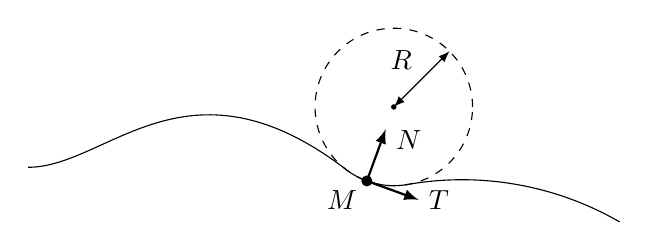
\begin{tikzpicture}
    \draw[dashed] ({4+1*sin(40)}, {1*cos(40)}) coordinate (C) circle(1);
    \draw (0,0) .. controls (1, 0) and (2, 1.5) .. (4, 0) arc(230:280:1)  arc(100:60:4);
    \coordinate (M) at ($(C)+(250:1)$); 
    \fill (C) circle(1pt);
    \fill (M) circle(2pt) node[below left]{$M$} ;
    \draw[latex-latex] (C) -- ++(45:1) node[midway, above left] {$R$}; 
    \draw[thick, -latex] (M) -- +(-20:0.7) node[right]{$\vv{T}$} ;
    \draw[thick, -latex] (M) --+(70:0.7) node[right, yshift=-4pt] {$\vv{N}$};
  \end{tikzpicture}
  \captionof{figure}{Vecteurs de base du repère de Frenet et rayon de courbure de la trajectoire.}
\end{center}

Par analogie avec le mouvement circulaire, on peut écrire les composantes du vecteur accélération d'un point $M$ dans le repère de Frenet :
\begin{equation}
  \vv{a} = \dt{v}\vv{T} + \frac{v^2}{R}\vv{N}
\end{equation}
Avec $v=\norm{\vv{v}}$ et $R$ est le \textbf{rayon de courbure}  de la trajectoire. Lorsque la trajectoire tourne dans le sens trigonométrique, le rayon de courbure est positif, sinon il est négatif.

Les caractéristiques du vecteur accélération sont donc les mêmes que pour un mouvement circulaire. 

\end{document}
